%____________________________________________________________________________||
\section{Event selection for signal and control regions}
\label{sec:selection}

This section first outlines the set of ``pre-selection'' requirements
that are common to all signal and control regions, before defining the
selection criteria that are specific to each region.

%%____________________________________________________________________________||
\subsection{Pre-selection}
\label{sec:preSelection}

{\bf Removing instrumental sources of ``fake'' \met.} 

A number of beam- and detector-related effects can induce significant
\met. Examples include beam halo, reconstruction failures, spurious
detector noise, or event misreconstruction due to detector
inefficiencies. These events, with large, non-physical values of \met,
are rejected with high efficiency by applying a range of dedicated
vetoes. All ``MET filters'' recommended by the JetMET POG and SUSY PAG
are applied by default in this analysis and listed in Table~\ref{tab:pre-selections}.

{\bf Jet requirements.} 

Jets considered in the analysis are required to satisfy $\PT>40\gev$
and $|\eta|<3.0$. Events containing jets in the forward region that
satisfy the requirements $\PT>40\gev$ and $|\eta|>3.0$ are rejected in
order to control background contributions from SM processes, without
introducing a significant reduction in signal acceptance. The jets
that are selected are used in the calculation of all jet-based
event-level variables, such as \HT, \mht, and \alphat.

Raised $\PT$ thresholds and tighter $\eta$ requirements on the lead jets 
are also required. The lead jet is required to satisfy $\PT > 100\gev$
and $|\eta|<2.5$. This helps to ensure high trigger efficiencies,
but also helps to improve the S/B for a wide
range of models with respect to SM processes, such as V + jets
production. Events are then classified based on the
second leading jet. In the case that a second leading jet satisfies $\PT > 100\gev$ 
events are assigned to a ``symmetric'' \njet category. If the second
jet satisfies $40 < \PT < 100\gev$ events are assigned to an
``asymmetric'' \njet category. Finally, if there is no second leading
jet with $\PT>40\gev$, events are assigned to the ``mono-jet''
category. The asymmetric and mono-jet categories have been added to
the analysis to help improve acceptance to a range of DM models and compressed
SUSY.

{\bf Event categorisation according to \njet and \nb.} 

Events in the hadronic signal and all control regions (described
below) are categorised identically and according to the number of jets
(\njet) reconstructed in each event and the number of jets identified
as originating from bottom quarks (\nb) in each event. As a baseline,
the resulting sub-samples comprise events containing exactly one, two,
three, four, or at least five jets. These are further split into
``monojet'' (only in the $\njet=1$ case),
``symmetric'' or ``asymmetric'' \njet categories according to the
second leading jet \Pt, as defined above.

Events are also categorised according to the the number of b-tagged
jets (``b-jets''). As a baseline, the sub-samples are defined by
requiring exactly zero, one, two, or at least three b-tagged jets. By
construction, $\nb \leq \njet$. Events containing three or more b-tags
typically implies either an additional source of b-jets beyond those
from the \ttbar process (\eg via gluon splitting) or at least one
mistag of a jet from a light-flavoured parton. The number of b-tagged
jets is currently taken directly from simulation.

%In the near future, the ``b-tag formula method'' (described below and
%detailed in Ref.~\cite{Chatrchyan:2013lya}) will again be employed to
%improve the statistical precision of predictions involving events
%containing high multiplicities of b-tagged jets, which will allow for
%the addition of further categories that contain at least four b-tagged
%jets. 

%In order to maximise sensitivity to potential new physics
%signatures in final states with a high b-quark content, a method that
%improves the statistical power of the predictions from simulation,
%particularly for $n_\cPqb \ge 2$, is employed~\cite{Chatrchyan:2013lya}. The
%distribution of $n_\cPqb$ is estimated from generator-level
%information contained in the simulation, namely the number of
%reconstruction-level jets matched to underlying bottom quarks
%($n_\cPqb^\text{gen}$), charm quarks ($n_\cPqc^\text{gen}$), and
%light-flavoured partons ($n_\cPq^\text{gen}$) per event. All relevant
%combinations of $n_\cPqb^{\rm gen}$, $n_\cPqc^{\rm gen}$, and
%$n_{\cPq}^{\rm gen}$ are considered, and event counts are recorded
%according to the categorisation of events in terms of \njet and
%\scalht. The efficiency $\epsilon$ with which b-quark jets are
%identified and the mistag probabilities $f_\cPqc$ and $f_\cPq$ are
%also determined from simulation per event category, with each quantity
%averaged over jet \pt and $\eta$. Corrections are applied on a
%jet-by-jet basis to $\epsilon$, $f_\cPqc$, and $f_\cPq$ in order to
%match the corresponding measurements from
%data~\cite{Chatrchyan:2012jua}. This information is sufficient to
%predict $n_\cPqb$ and thus also determine the event yield from
%simulation for a given event category. The event yields for a given
%b-quark jet multiplicity can be predicted with a higher statistical
%precision than obtained directly from simulation, particularly for
%events with high counts of b-quark jets.

{\bf \HT,\mht requirements and binning.} 

Events are required to have significant hadronic activity by requiring
$\scalht > 200\GeV$. Despite an increase in both multijet production
cross sections and pileup in Run~2, the lowest \HT threshold is
kept at the same value of the Run~1 analysis~\cite{Chatrchyan:2013lya}
in order to maintain acceptance to DM models or compressed
SUSY. Events in all samples are binned identically, according to the
\HT variable. The choice of binning in \HT is driven primarily by the
trigger strategy employed by the analysis, as described in
Section~\ref{sec:triggers}, and can be summarised as follows: 50\gev
bins in the range $200 < \HT < 400\gev$, 100\gev bins in the range
$400 < \HT < 600\gev$, a 200\gev bin $600<\HT<800\gev$ and a final 
inclusive bin $\HT > 800\gev$.

Events are also required to have appreciable missing hadronic energy
by requiring $\mht>130\gev$. This ensures that all events used within
the analysis have a degree of missing energy similar to that required
in the signal region via an \alphat cut. This is outlined in
Sec.~\ref{sec:had-signal}. 

The lower threshold of the last (inclusive) \HT bin is not forced to
$800\gev$, it is instead determined
independently for each (\njet,\nb) event category and is chosen to
always align with one of the ``default'' boundaries defined above. The
metric for choosing the final bin threshold is based on the number of
events in the corresponding event category and \HT bin of the data
control samples. This ensures that all bins in the data control
samples are sufficiently populated to ensure a statistically
significant prediction in each of the corresponding signal region
bins. Currently, this is achieved by requiring at least $10$ predicted
events in each \HT and \njet category of the control regions
along with the requirement that there is at least one observed
event per \nb category. If this is not the case, events from high \HT bins are combined
into a single inclusive bin that satisfies this metric. This metric
ensures that there are sufficient events in the control samples
to probe for potential systematic effects with closure tests between
simulation and data, as described in Sec.~\ref{sec:systematics}.

\begin{table}[h!]
  \topcaption{Summary of the pre-selection criteria.}
  \label{tab:pre-selections}
  \centering
  \footnotesize
  \begin{tabular}{ ll }
    \hline
    \hline
    Selection                     & Requirement                                                                          \\
    \hline
    ``MET filters''               & Primary Vertex, CSC Beam Halo, HBHE Noise and Isolation, ECAL Endcap SC Noise        \\
    Jet acceptance                & $\PT > 40\gev$, $|\eta| < 3$                                                         \\
%    \njet                         & $\geq2$                                                                \\
    Lead jet acceptance           & $\PT > 100\gev$, $|\eta| <    2.5$                                     \\
    Second jet acceptance         & $\PT > 100\gev$ \texttt{OR} $40 < \PT < 100\gev$                       \\
    Loosest \HT requirement       & $\HT > 200\gev$                                                        \\
    Loosest \mht requirement      & $>130\gev$                                                     \\  
    Baseline \HT binning          & 200--250, 250--300, 300--350, 350--400, 400--500, 500--600, 600--800, $>$800\gev \\
    Baseline \njet multiplicities & 1 (mono-jet), 2, 3, 4, $\geq$5 (both symmetric and asymmetric)                       \\
    Baseline \nb multiplicities   & 0, 1, 2, $\geq3$ ($\nb \leq \njet$)                                    \\
    \hline
    \hline
  \end{tabular}
\end{table}

{\bf Summary of pre-selection requirements.} 

Table~\ref{tab:pre-selections} summarises the pre-selection
requirements and default categorisation and binning scheme. The
threshold of the final \HT bin per (\njet,\nb) category is summarised
in Table~\ref{tab:binning-3fb}. An identical scheme is used for the
signal region and all control regions. No extrapolation is performed
in the variables \njet, \nb, and \HT in this analysis. For each of the
signal and control regions, thirty event categories are considered,
each with up to seven bins in \HT, assuming an integrated luminosity
of 2.1\ifb. 

\begin{table}[h!]
  \caption{Threshold (GeV) of the final \HT bin as a function of event
    category (\njet,\nb), which is always aligned with respect
    to one of the baseline boundaries (motivated primarily by the trigger) of
    200, 250, 300, 350, 400, 600, 800\gev. 
    %This is the projected choice for 3\fbinv.
    }
  \label{tab:binning-3fb}
  \centering
  \footnotesize
  \begin{tabular}{ l|cc|ccc|cccc|cccc|cccc }
    \hline
    \hline
    \njet      & \multicolumn{2}{c}{1} $ \multicolumn{3}{c}{2} & \multicolumn{4}{c}{3} & \multicolumn{4}{c}{4} & \multicolumn{4}{c}{$\geq5$}                                                   \\ 
    \nb        & 0                     & 1                     & 0                     & 1                     & 2                     & 0   & 1   & 2   & 3   & 0   & 1   & 2   & $\geq3$ & 0   & 1   & 2   & $\geq3$ \\
    \hline
    Symmetric  & 600                   & 500                   & 800                   & 800                   & 600                   & 800 & 800 & 800 & 400 & 800 & 800 & 800 & 800     & 800 & 800 & 800 & 800     \\
    Asymmetric & -                     & -                     & 600                 & 500                   & 400                   & 600 & 600 & 500 & 300 & 600 & 600 & 600 & 400     & 600 & 600 & 600 & 500     \\
    \hline
    \hline
  \end{tabular}
\end{table}

%{\bf Evolution of event categorisation and \HT binning versus integrated luminosity.} 

%The choice of how events are categorised according to the number of
%\njet and \nb and binned in \HT will evolve as a function of
%integrated luminosity. Additional categories with higher jet
%multiplicities maybe added for data samples corresponding to higher
%integrated luminosities (\eg $\sim$10\fbinv). Additional categories
%with higher b-tag multiplicities will also be considered once the
%b-tag ``formula method''~Ref.~\cite{Chatrchyan:2013lya} has been commissioned with data. This
%will allow for categories defined by the requirement of at least four
%b-tagged jets. Additional bins at high \HT will also be considered for
%higher integrated luminosity scenarios. 

\subsection{Lepton and photon vetoes \label{sec:vetoes}}

To select a sample of events in the hadronic final state and to
suppress SM processes with genuine \met from neutrinos, events
containing an isolated electron with $\pt > 10\GeV$ and $|\eta| < 2.5$
or an isolated muon with $\pt > 10\GeV$ and $|\eta| < 2.5$ are
vetoed. Further, to reduce the ``lost leptons'' backgrounds from \wj
and \ttbar, events containing single isolated tracks with $\pt >
10\GeV$ and $|\eta| < 2.5$, as defined in Sec.~\ref{sec:objects},
are vetoed as part of the signal region selection criteria. In the
case of the single and di-lepton control samples, a further
requirement is made such that events are not vetoed due to the
presence of a track from the well identified leptons, by requiring
$\Delta R(\textrm{track},\textrm{lepton}) > 0.02$.

Finally, to select a purely hadronic topology and to allow for a
orthogonal control region, events are vetoed in which an isolated photon
with $\pt > 25\GeV$ and $|\eta| < 2.5$ is identified.

\subsection{The hadronic signal region}
\label{sec:had-signal}

The lepton and photon vetoes are applied to select hadronic final
states. All pre-selection criteria are also applied. Following these
selections, the multijet background from QCD is still several orders
of magnitude larger than the typical signal expected from SUSY.

{\bf \HT-dependent \alphat requirements.}

Background events from multijet production populate the region
$\alphat \lesssim 0.5$ and therefore can be rejected with very high
efficiency by requiring an appropriate cut on \alphat. In the Run~1
analyses, a minimum requirement of $\alphat > 0.55$ was imposed, with
a raised threshold (as high as 0.65) used at low \HT to control
against a potential increase in contamination from multijet production
due to worsening resolution and jet \PT threshold effects.  (The
latter effect refers to ``fake'' \mht arising from the rare occurrence
of multiple soft jets below threshold that are relatively collinear.)
The minimum threshold of 0.55 was motivated primarily by the control
of the multijet background and considered conservative for mid to high
regions in \HT, while maintaining good signal acceptance. However,
improving jet resolutions and a reduced jet threshold effect relative
to an increasing \HT scale means that looser \alphat thresholds can be
used at higher values of \HT.

A useful approximate conversion between \alphat and \mht can be
obtained by calculating \alphat, as described by Eq.~\ref{eq:alphat3}, 
while forcing $\dht = 0\gev$,. Hence, using this metric, the
dependence of the \alphat requirement as a function of the \HT bin can
be determined such that the effective requirement on \mht is
comparable, \ie roughly constant, across all \HT bins. The values
typically fall in the range $\sim110 < \mht < \sim160\gev$. This
approximate levelling of the ``effective'' \mht threshold implies
increasingly tighter requirements against instrumental effects versus
\HT, while maximising signal
acceptance. Table~\ref{tab:alphat-thresholds} summarises the expected
\alphat thresholds and corresponding ``effective'' \mht thresholds for
each \HT bin. The \alphat threshold is dependent only on \HT and not
on \njet nor \nb that are used to define the event categories.

\begin{table}[h!]
  \caption{\alphat and corresponding ``effective'' \mht (GeV) thresholds versus
    lower bound of \scalht bin. For all \HT bins satisfying $\HT > 800
    \gev$, the direct requirement of $\mht > 130\gev$ is imposed rather
    than a requirement on \alphat. No \alphat requirement is imposed in the
    monojet bins.}
  \label{tab:alphat-thresholds}
  \centering
  \footnotesize
  \begin{tabular}{ lcccccccc }
    \hline
    \hline
    \scalht            & 200       & 250       & 300       & 350       & 400       & 500       & 600       \\
    \hline                                                                                     
    \alphat threshold  & 0.65      & 0.60      & 0.55      & 0.53      & 0.52      & 0.52      & 0.52      \\
    ``Effective'' \mht & $\sim$128 & $\sim$138 & $\sim$125 & $\sim$123 & $\sim$110 & $\sim$138 & $\sim$162 \\
    \hline
    \hline
  \end{tabular}
\end{table}

For Run~2, all signal region bins satisfying $\HT > 800\gev$ are
seeded by the single-object \texttt{HLT\_HT800} trigger, which is
expected to be unprescaled. For these high \HT bins, no \alphat
threshold is required, which removes the inefficiencies of this
variable for high jet multiplicity events. Instead, the following
$\mht >130\gev$ requirement helps to control the multijet background
along with the imposition of $\bdphi > 0.5$ (described below).

{\bf \bdphi requirement.} 

Further, an additional powerful variable \bdphi is used to suppress
multijet contamination due to both instrumental effects and
semi-leptonic heavy-flavour decays with genuine \met in the final
state. The variable is determined as follows. The jet-based estimate
of the missing transverse energy, ${\mhtvec}$, is recomputed while
ignoring one of the reconstructed jets (the ``test'' jet). The
difference in the azimuthal angle between the recomputed $\mhtvec$
and the ``test'' jet is then determined. This process is repeated for
each jet in the event and the minimum of all the azimuthal
differences, \bdphi, is determined. For monojet events, the calculation is 
performed using all jets with $\Pt > 20\gev$. The ``test'' jet whose subtraction
from the calculation $\mhtvec$ yields this minimum value, is
identified as the jet that is most likely to have given rise to the
missing transverse energy in the event. Events with significant \mht
due to instrumental effects or heavy flavour decays populate the
region $\bdphi \approx 0$ and so candidate signal event are accepted
only if they satisfy $\bdphi > 0.5$. The use of the \bdphi and \alphat
variables provide an extremely powerful rejection factor against
contamination from multijet events and allow to maintain low jet \PT,
\HT, and \mht thresholds, which in turn maximises signal acceptance
for a large range of DM and SUSY models with final states
characterised by the presence of significant \met.

{\bf $\mht/\met$ cleaning filter.} 

To protect against multiple jets failing the $\Et$ threshold or
falling out of detector acceptance, the jet-based
estimate of the missing transverse energy, \mht, is compared to the
missing transverse energy variable, $\met$, and events with $R_{\rm
  miss}=\mht/\met > 1.25$ are rejected.
  
{\bf Detector dead cell control.}

Masked regions in the ECAL (which amount to about 1\% of the ECAL channel count)
or HCAL, or by missing instrumentation in the barrel-endcap gap, could cause 
severe energy losses. A data-driven method is developed to identify dead cells. The 
procedure is carried out on events that pass a loose selection of one good primary vertex,
$\njet>1$ and $\scalht>150\gev$. For each identified jet with
$\PT > 20 \gev$ in data, the azimuthal angle ($\Delta\phi_{jet}$) between the jet and the 
recomputed ${\mhtvec}$ is determined, in the same way as in the procedure to compute the \bdphi 
variable. The positions of all jets which give $\bdphi < 0.3$ are plotted in
an $\eta-\phi$ map. Subsequently, the positions of all jets with
$\pt>20\gev$ are plotted in a second $\eta-\phi$ map.
These two maps are then divided to form a 2D ratio map, taking the
first map as the numerator and second as the denominator.
Jets pointing to dead cells are likely to give $\bdphi < 0.3$, so the
location of dead cells in $\eta$ and $\phi$ have higher values in this 2D ratio map. 

Figure~\ref{fig:2dRatioMap} is the 2D ratio map made with unblinded signal region with luminosity of 
149.49~$\text{pb}^{-1}$. In the lower left region of the plot, two
areas with significant instrumental effects are clear. To ensure these
effects are filtered out by all cleaning cuts within the analysis, an
$\eta-\phi$ map of all jets with $\pt>20\gev$ and $\bdphi<0.3$ are
plotted after the signal region selection (as described in
Sec.~\ref{sec:had-signal}), shown in
Fig.~\ref{fig:jetMapPostSignalSelection}. The areas with significant
instrumental effects visible in Fig.~\ref{fig:2dRatioMap} do not appear
to remain in Fig.~\ref{fig:jetMapPostSignalSelection}. This implies the current suite of cleaning cuts
is enough to remove any localised detector effects.

\begin{figure}[h!]
    \begin{center}
        {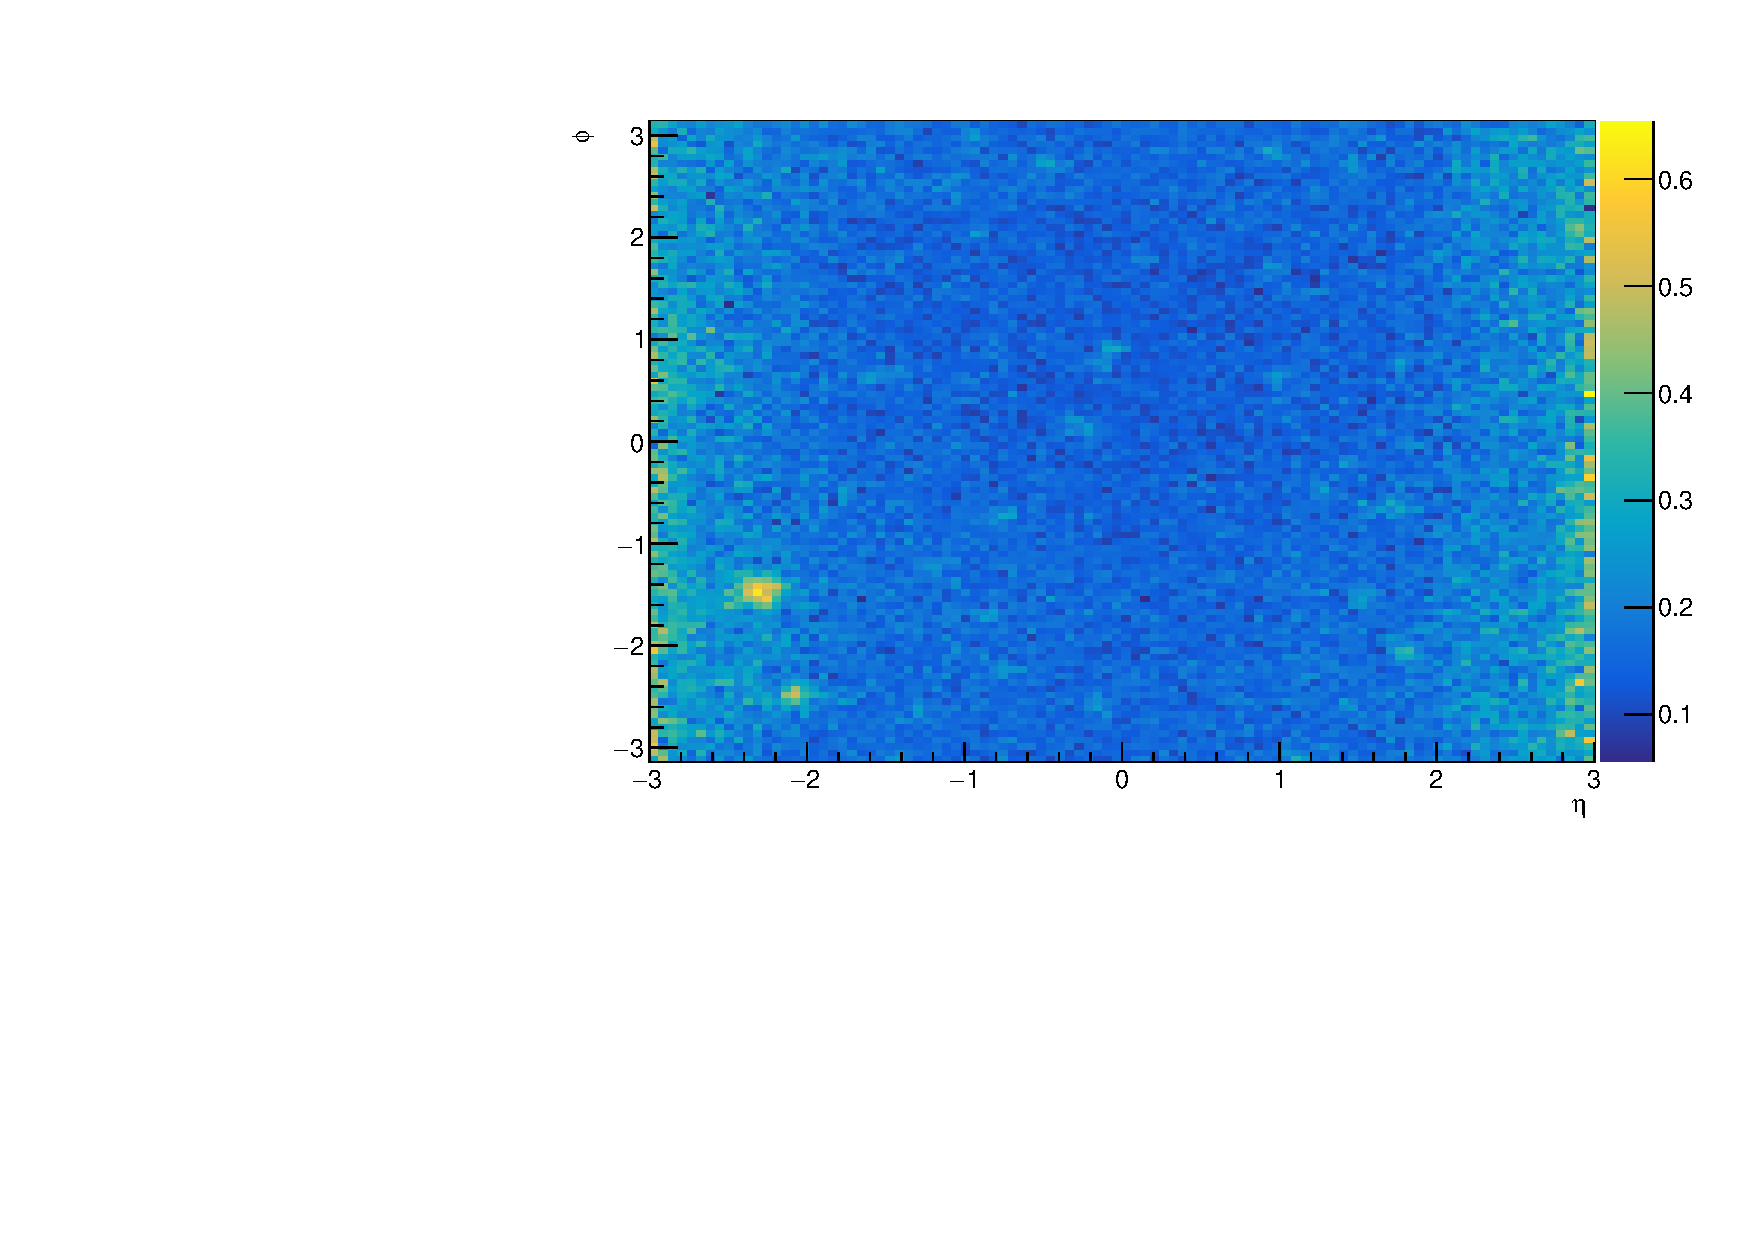
\includegraphics[width=0.7\textwidth]{figures/selection/EtaPhiMap.pdf}}
        \caption{The 2D ratio of jets ($\pt>20\gev$) with $\bdphi<0.3$ plotted in the
        $\eta-\phi$ plane, divided by all jets that satisfy $\pt>20\gev$. 
        Made with 149.49~$\text{pb}^{-1}$ of
        events that pass a loose selection of one good primary vertex,
        $\njet>1$ and $\scalht>150\gev$.}
        \label{fig:2dRatioMap}
    \end{center}
\end{figure}

\begin{figure}[h!]
    \begin{center}
        {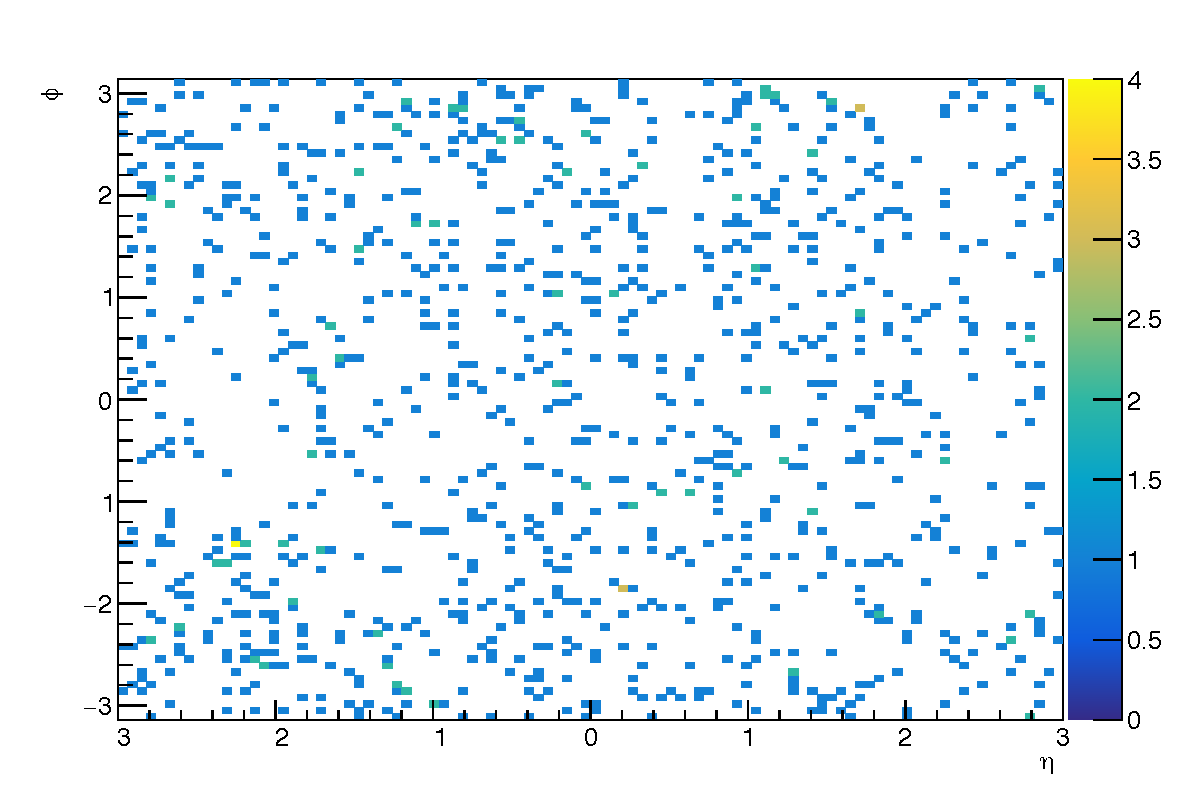
\includegraphics[width=0.7\textwidth]{figures/selection/bDPhilt0p3AfterSelection.pdf}}
        \caption{Jets ($\pt>20\gev$) with $\bdphi<0.3$ plotted in the
        $\eta-\phi$ plane. 
        Made with $1.26\ifb$ of
        events that pass the full signal region selection.}
        \label{fig:jetMapPostSignalSelection}
    \end{center}
\end{figure}

%To protect against severe energy losses caused by masked regions in the ECAL (which
%amount to about 1\% of the ECAL channel count) or HCAL, or by missing
%instrumentation in the barrel-endcap gap, events with $\bdphi < 0.5$
%are rejected if the distance in the ($\eta,\phi$) plane between the
%selected jet and the closest masked ECAL region, $\Delta R_{\rm
%  ECAL}$, is smaller than 0.3. Similarly, events are rejected if the
%jet points within 0.3 in $\eta$ of the ECAL barrel-endcap gap at
%$|\eta| = 1.5$.

{\bf Beam halo.}

The CSC beam halo filter has been found to be less efficient during the early
Run 2 data-taking period compared to the previous run.

Beam halo events manifest themselves as single energy deposits in the
calorimeters, which introduces large amounts of ``fake'' \met. This effect is
especially prominent in the signal region monojet category, particularly at
$\phi$ coordinates of 0 and $\pi$ because of the tendency of halo particles to
lie within the plane of the LHC ring. This is evident in
Fig.~\ref{fig:leadJetCleaning}.

Such spurious events are suppressed by requiring at least 10\% of the leading
jet's energy to originate from charged hadrons, $CHF>0.1$. The effectiveness of this selection
is demonstrated in Fig.~\ref{fig:leadJetCleaning}.

Beyond the filter available in the data ntuples, the JetMET POG have
provided lists of events that should fail the CSC beam halo and bad
ECAL super cluster filters. These extra events are vetoed and the
efficiency of events in the signal region (Sec.~\ref{sec:had-signal})
and single muon control region (Sec.~\ref{subsec:mucontrolSelection})
that pass this veto for each analysis bin are plotted in
Fig.~\ref{fig:cscFilterEfficiencies}. In the vast majority of bins the
extra filters are $100\%$ efficient, with a few bins with an
inefficiency at the $2-3\%$ level. This confirms that the $CHF$ cut is
already effectively removing spurious events that are present due to
beam halo effects. 

\begin{figure}[h!]
    \begin{center}
        {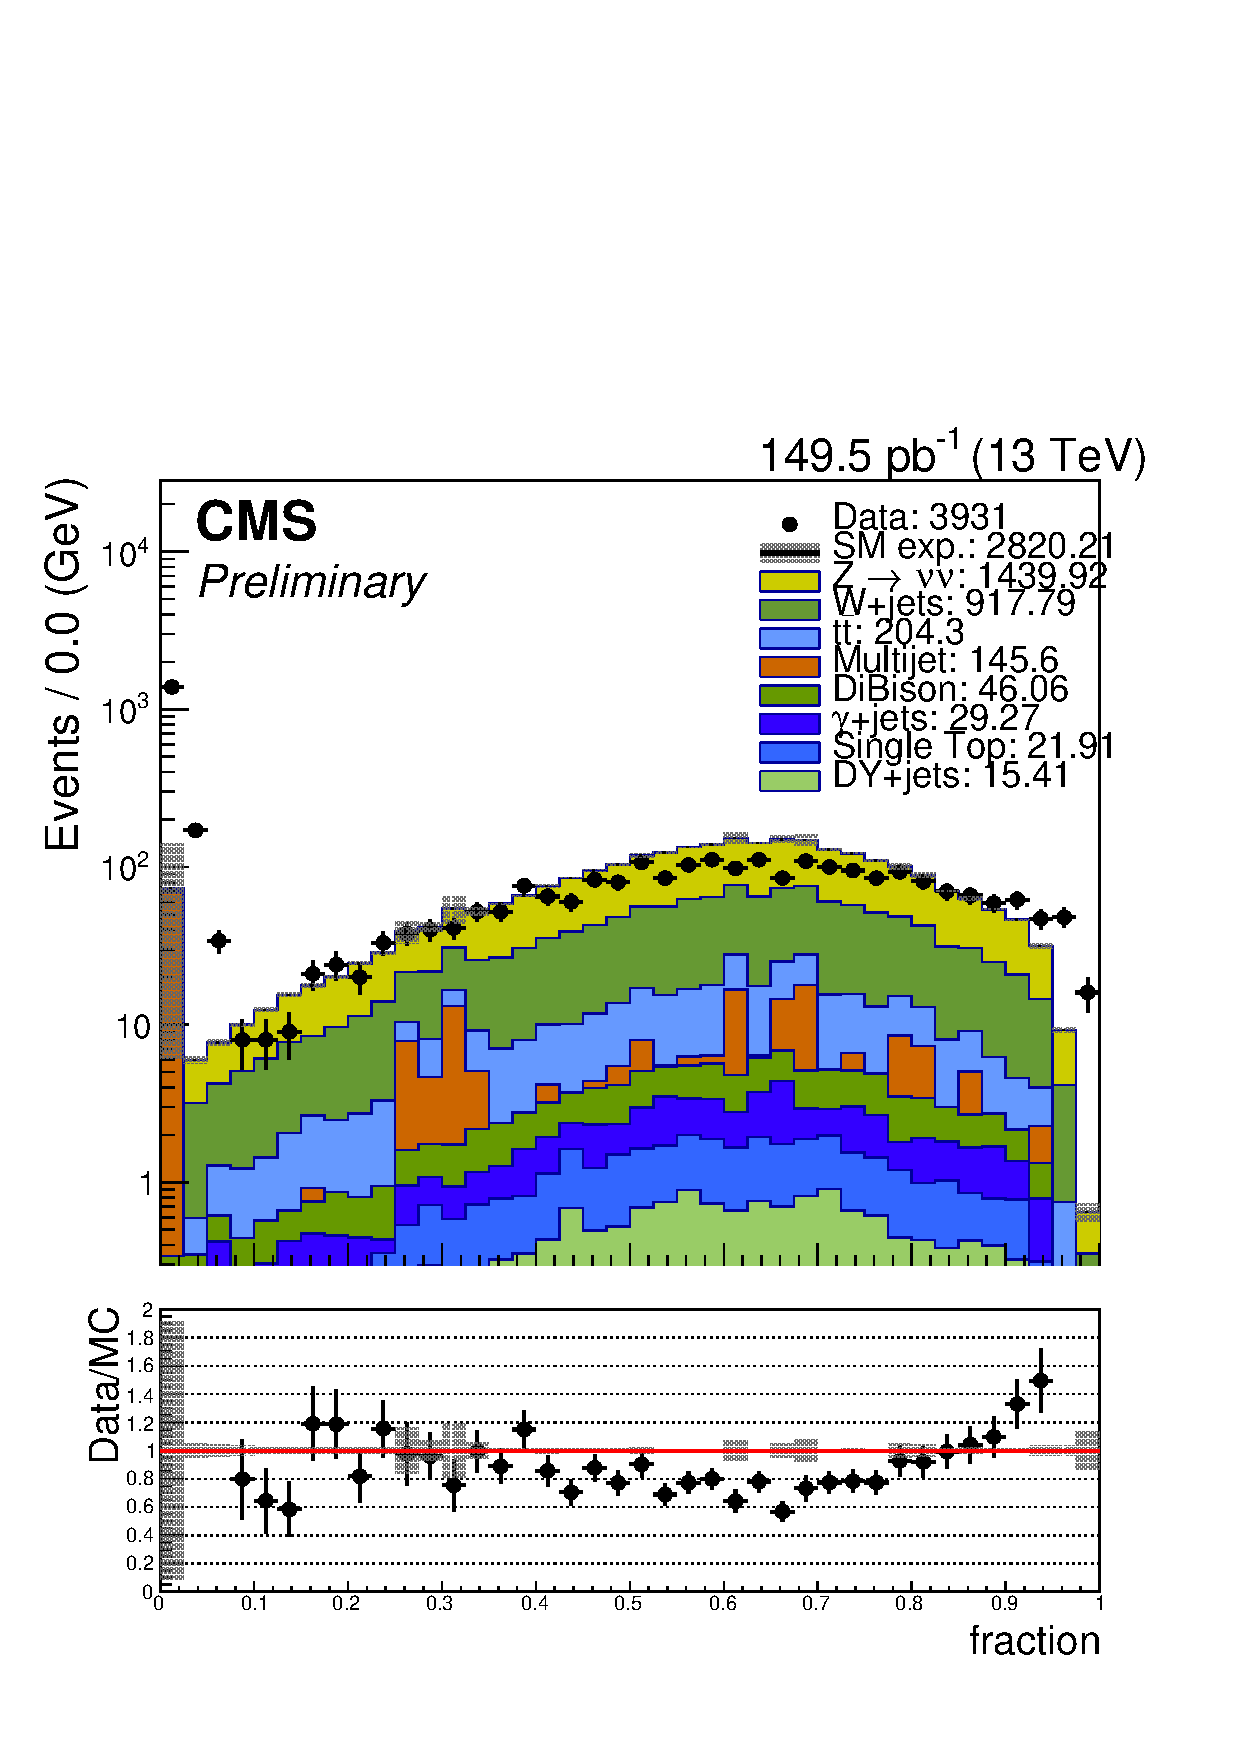
\includegraphics[width=0.32\textwidth]{figures/selection/leadJetChf_all_before.pdf}}
        {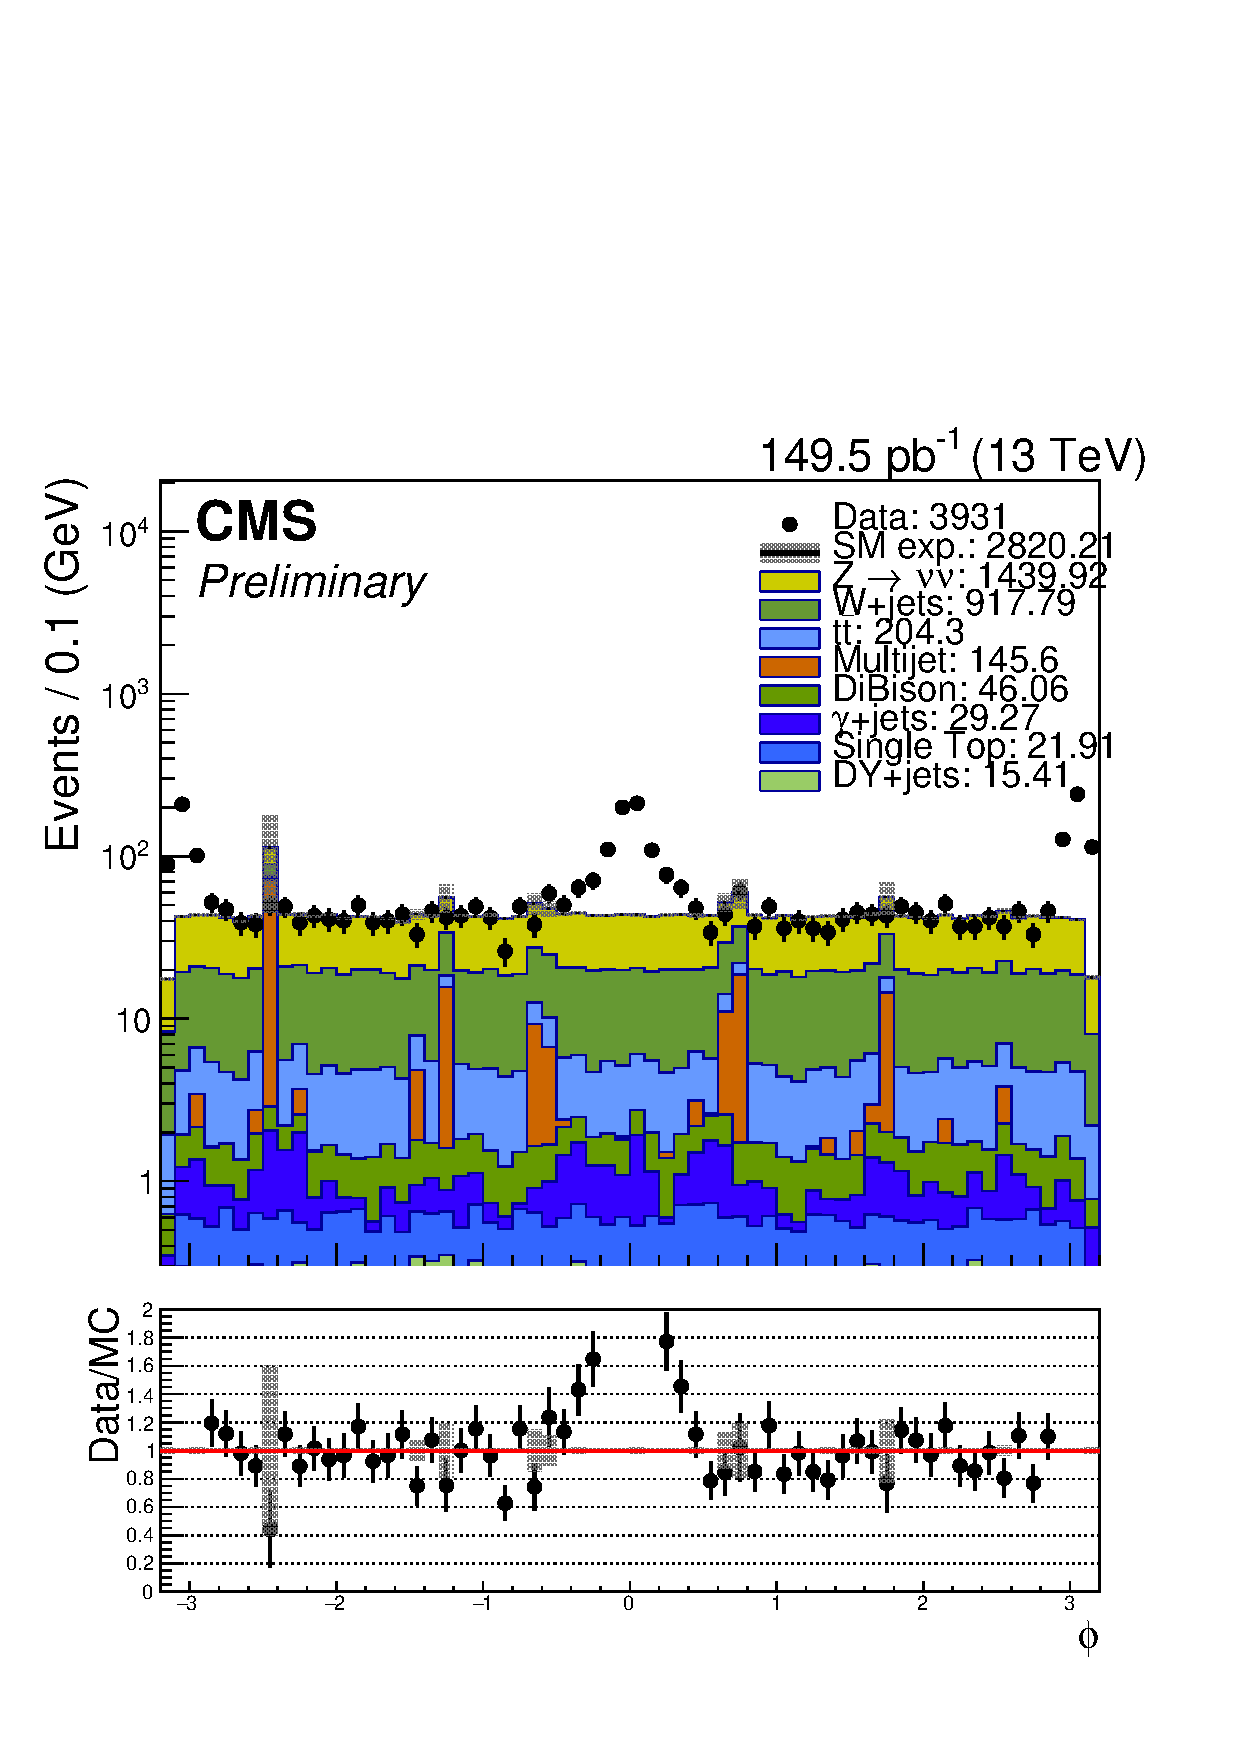
\includegraphics[width=0.32\textwidth]{figures/selection/leadJetPhi_all_before.pdf}}
        {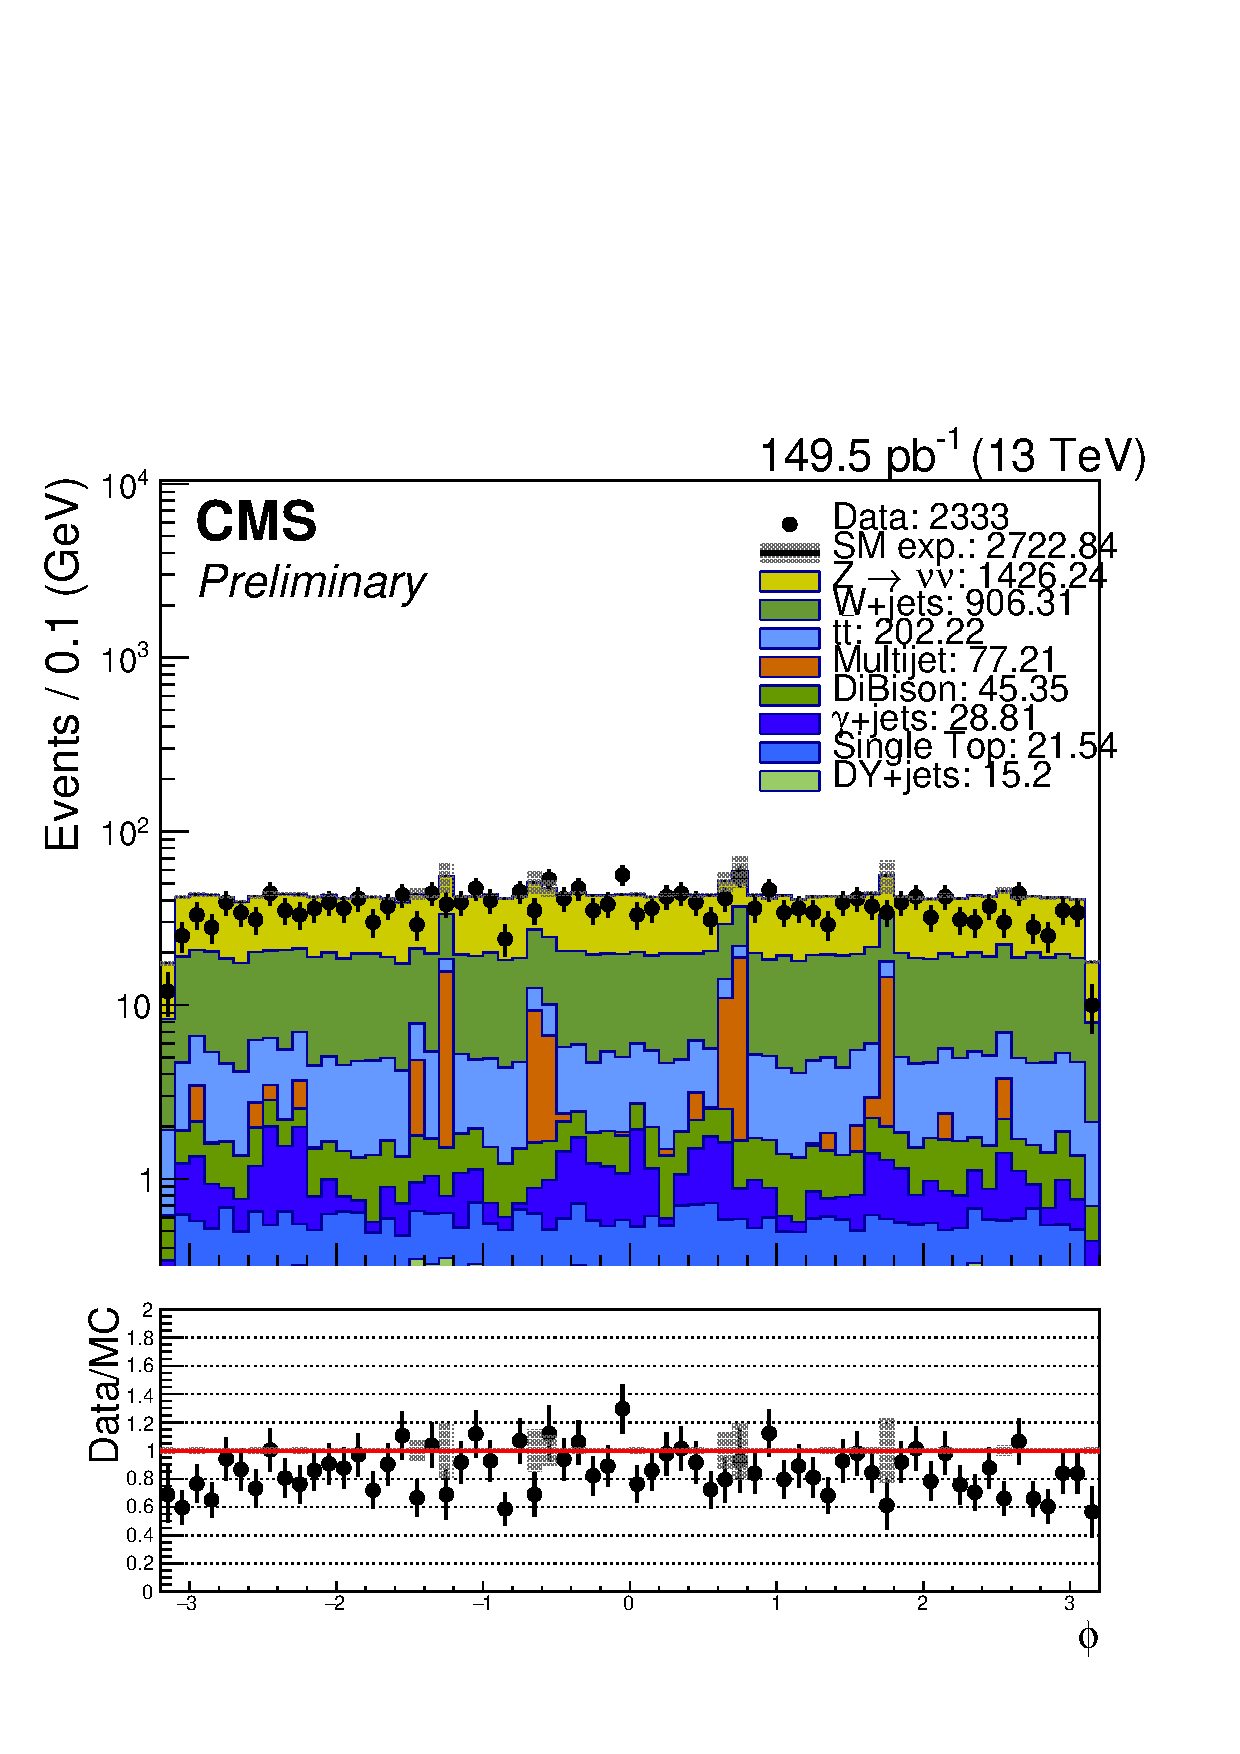
\includegraphics[width=0.32\textwidth]{figures/selection/leadJetPhi_all_after.pdf}}
        \caption{Distributions in the signal region of the lead jet charged hadron
        energy fraction (CHF) (Left), lead jet $\phi$ direction (Centre), and lead jet $\phi$
        direction after applying a requirement of {CHF~$>0.1$}. The large excess in data
        at charged hadron fractions close to zero and ${\phi = 0, \pi}$ is consistent with beam
        halo effects, and is effectively suppressed by the aforementioned selection.}
        \label{fig:leadJetCleaning}
    \end{center}
\end{figure}

\begin{figure}[h!]
  \begin{center}
    \subfigure[Signal region
    selection]{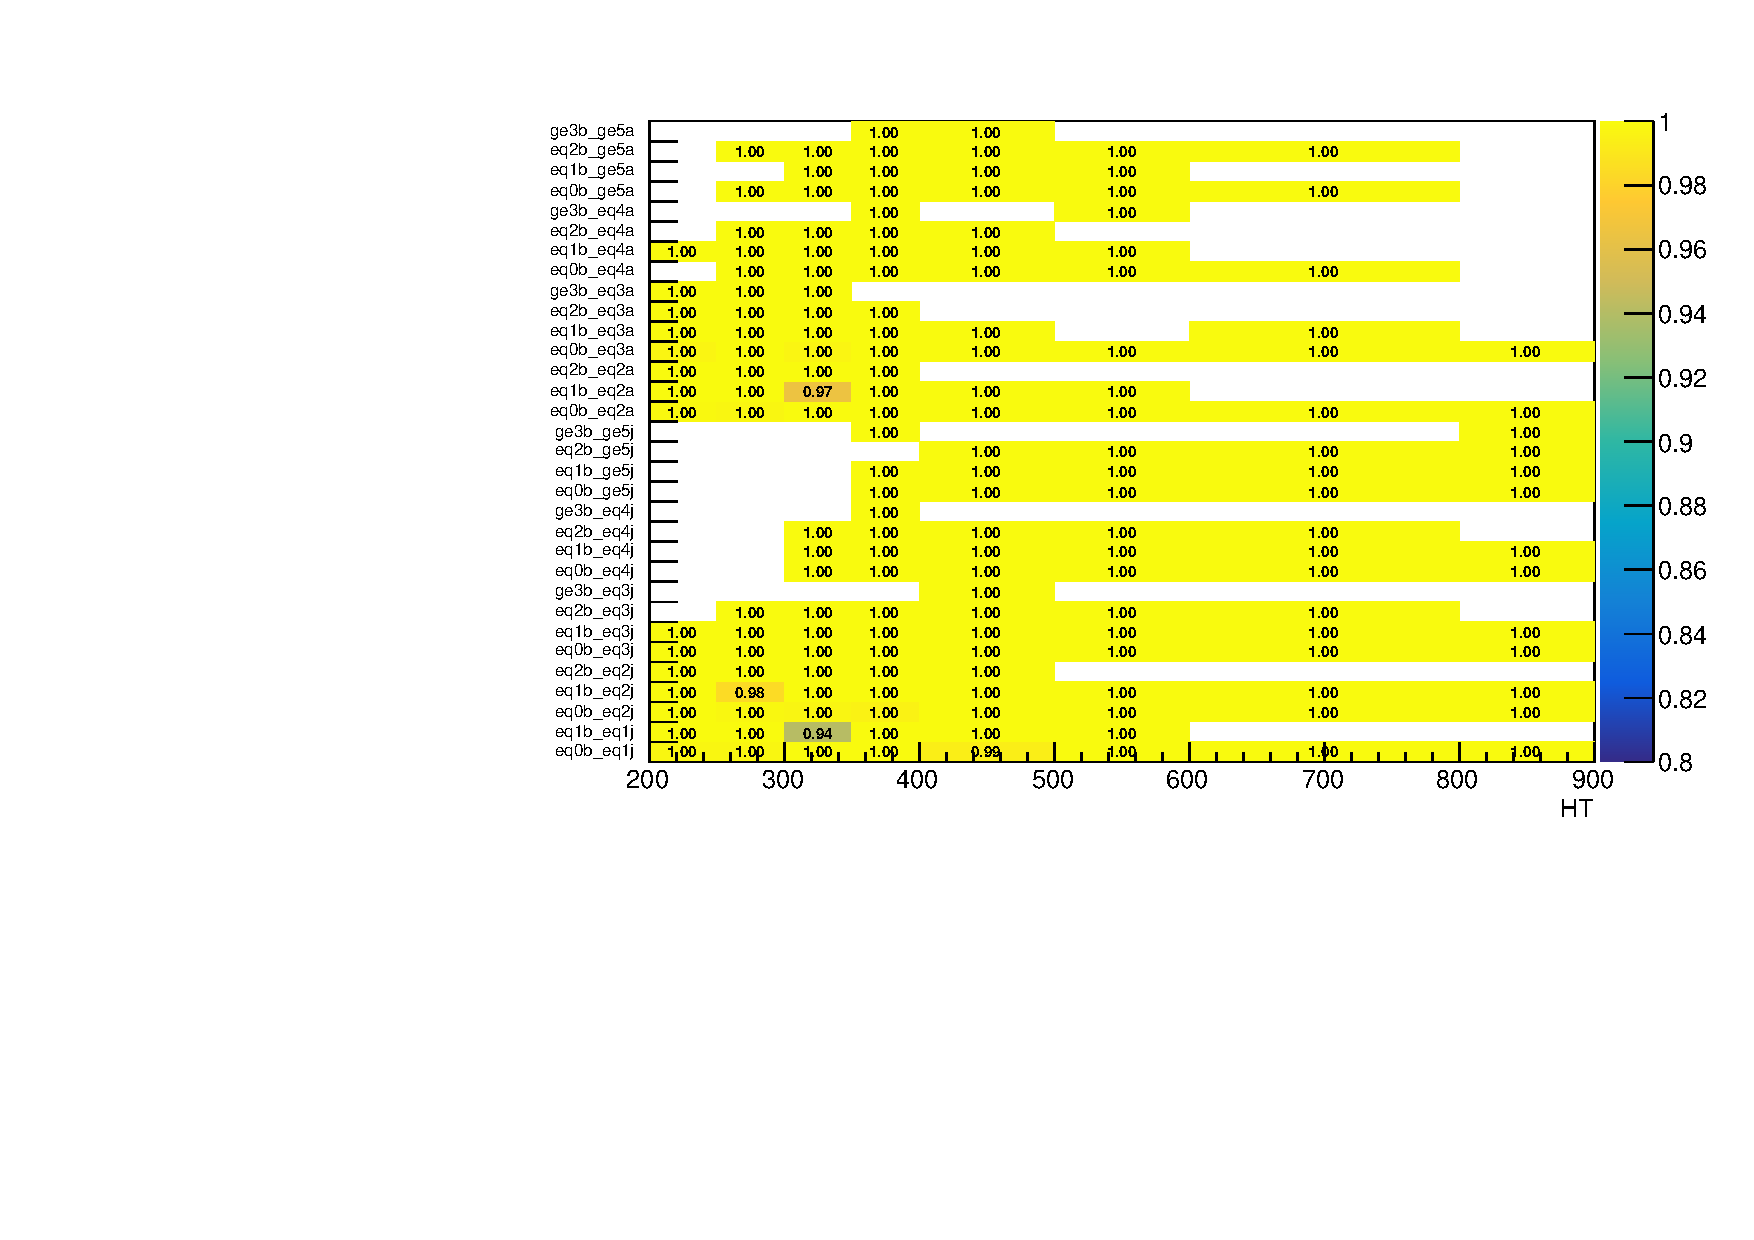
\includegraphics[width=0.5\textwidth]{figures/selection/Signal_Data_CSCEfficiency.pdf}} ~~
    \subfigure[Single muon control region
    selection]{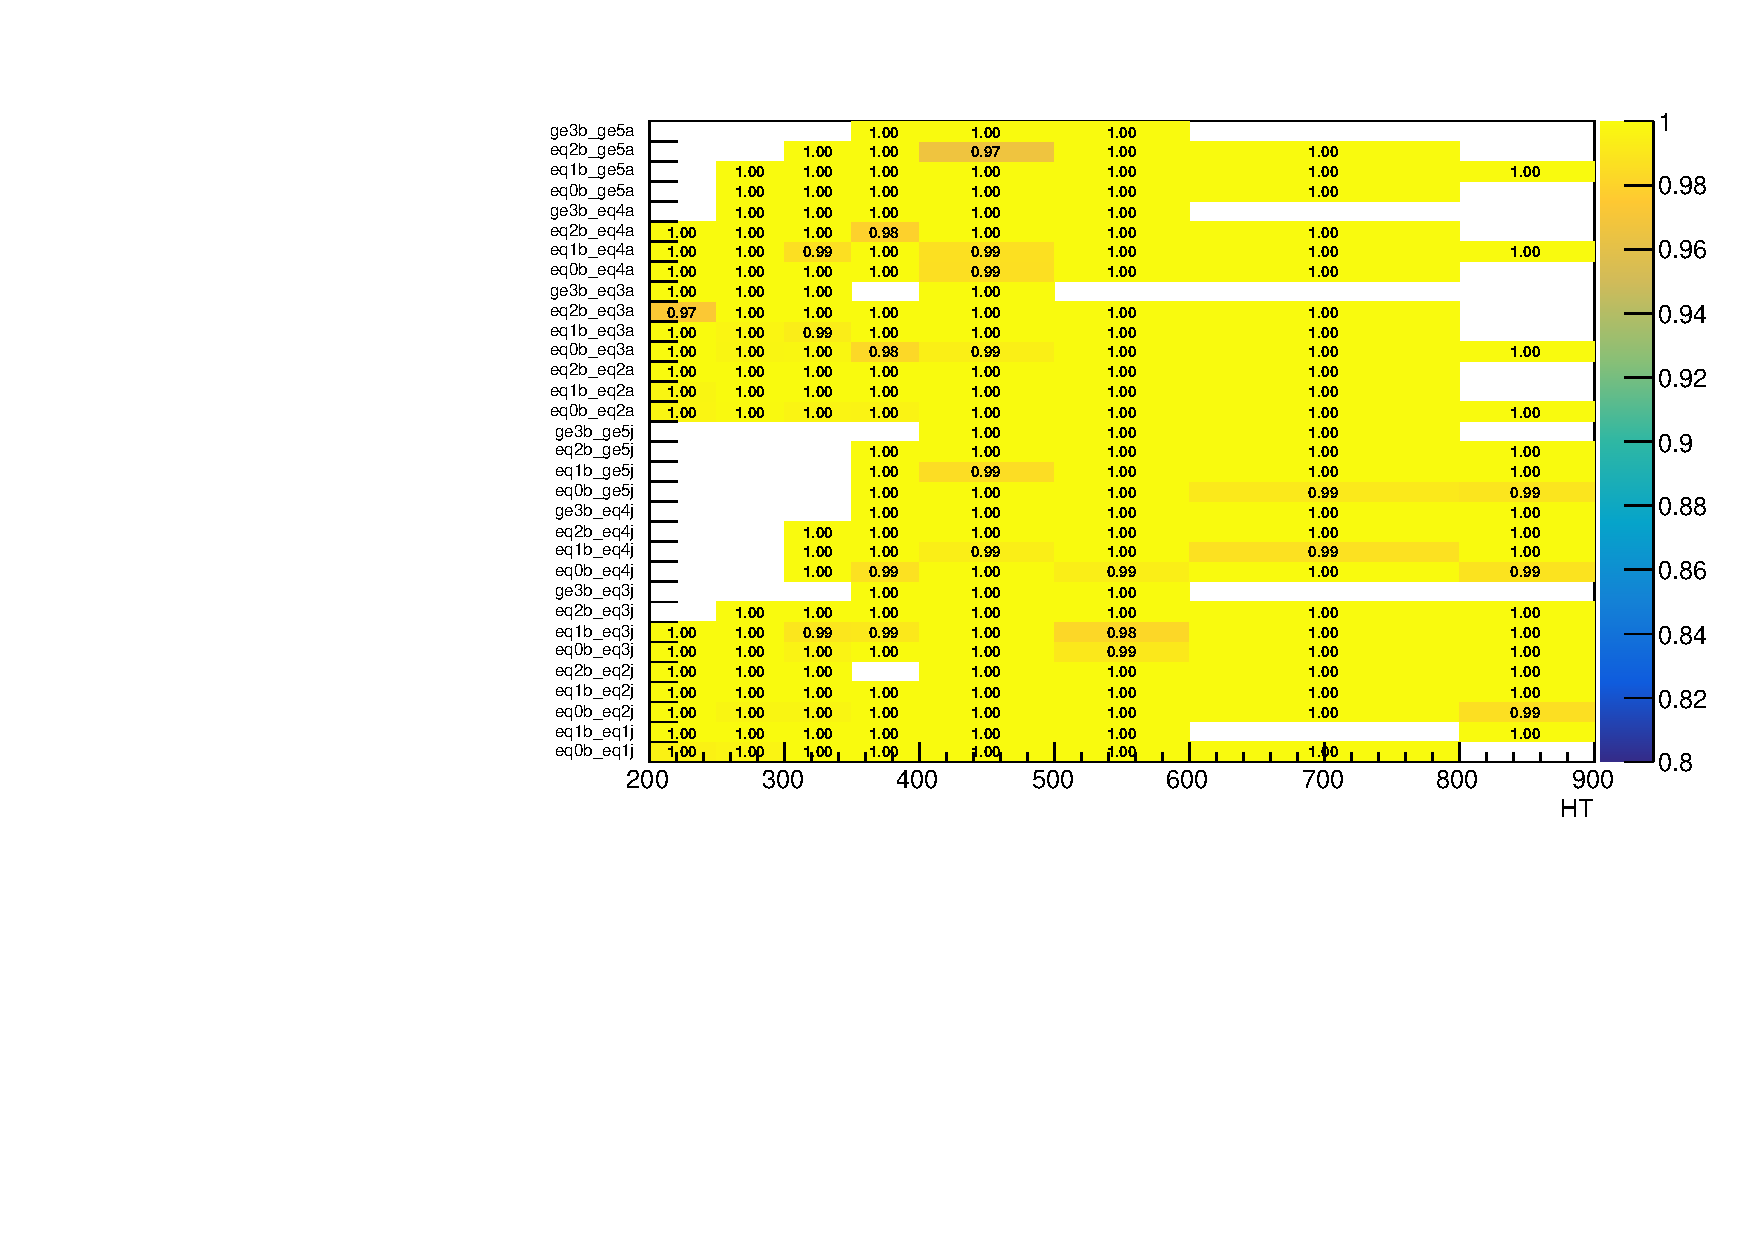
\includegraphics[width=0.5\textwidth]{figures/selection/SingleMu_Data_CSCEfficiency.pdf}} \\
    \caption{Efficiencies of the CSC beam halo and bad ECAL super
    cluster filters applied on $1.26\ifb$ of data passing the single
    muon and signal region selections.}
    \label{fig:cscFilterEfficiencies}
  \end{center} 
\end{figure}

{\bf Summary of signal region selection.} 

The requirements that define the hadronic signal region are summarised
in Table~\ref{tab:sr-selections}.

\begin{table}[h!]
  \topcaption{Summary of the signal region selection criteria, applied
    in addition to the pre-selection summarised in
    Table~\ref{tab:pre-selections}.}
  \label{tab:sr-selections}
  \centering
  \footnotesize
  \begin{tabular}{ ll }
    \hline
    \hline
    Selection             & Requirement                                                    \\
    \hline
    \alphat               & $>$0.52--0.65 (\HT-dependent) for region $200 < \HT < 800\gev$ \\
    \bdphi                & $>0.5$                                                         \\
    \mht/\met             & $<1.25$                                                        \\
    ``Dead ECAL filter''  & (see text)                                                     \\
    ``Beam Halo Filter''  &  $CHF(\textrm{leading jet})>0.1$                                \\

    \hline
    \hline
  \end{tabular}
\end{table}

\subsection{Adding the \texorpdfstring{\mht}{MHT} dimension}
\label{sec:had-shape}

As described above, and as used in Run~1, the analysis takes advantage
of three discriminating variables, \njet, \nb, and \HT, to provide
sensitivity to a large range of SUSY (and DM) models. No extrapolation
in these variables is performed, with predictions of SM background
yields in the (\njet,\nb,\HT) bins of the signal region based on both
observed counts and transfer factors derived from simulated yields in
the corresponding (\njet,\nb,\HT) bins of the control samples. Each
prediction is statistically and systematically independent.

In Run~1, for each (\njet,\nb,\HT) bin in the signal region, an
extrapolation in the variable \alphat was necessary to obtain
background predictions based on the muon control samples, which did
not impose any \alphat requirement. No extrapolation in \alphat was
performed for the photon control sample, which used the same \alphat
requirements as the signal region. The \alphat requirements used in
Run~1 for the signal region correspond loosely to \mht thresholds in
the range $\sim$130 to $\sim$500\gev depending on the \HT
bin. Uncertainties in this extrapolation were determined through
closure tests with respect to data, including one dedicated to the
\alphat extrapolation, plus additional cross checks.

In Run~2, we additionally bin event counts in the signal region
according to the variable \mht in order to provide further
discriminating power between any potential signal and the SM
background counts. Hence, while no extrapolation is performed in
\njet, \nb, nor \HT, the analysis relies on information obtained
from simulation to extrapolate from counts (integrated over \mht) in
the control samples to a predicted distribution in \mht for each
corresponding (\njet,\nb,\HT) bin in the signal region.

The \mht dimension is included in the likelihood model by using
templates determined per (\njet,\nb,\HT) bin from simulation. The
templates use an \mht bin width of 50\gev. The threshold of the final
\mht bin used by the templates is determined based on the size of the
available simulated samples: a statistical uncertainty of not more
than 50\% for the sum of all SM background processes is required. An
associated normalisation nuisance is determined from closure tests
between simulation and data, as described in
Sec.~\ref{sec:syst-on-shape}. Alternative templates are used to encode
the systematic uncertainty in the \mht distribution obtained from
simulation.

\subsection{The hadronic control region}

A hadronic control region that is enriched in multijet events and
disjoint with respect to the signal region is obtained by applying
both the pre-selection criteria and lepton/photon vetoes, as defined
above, and inverting the (\HT-dependent) \alphat and/or \mhtmet
requirements. 
%None of the cleaning filters are not applied to allow the study of
%instrumental effects. 
The sample of events populating this control region are used primarily
to estimate any residual background contamination from QCD multijet
events, described in Sec.~\ref{sec:qcd}.

\subsection{Commonalities between the data control regions}

There are five control regions with leptons or photons in the final
state: \mj, \mmj, and \gj. 
%\ej, \eej, and \gj. 
The full pre-selection is applied as part of the definition of each of these control
regions. The cuts on event-level jet-based quantities are identical to
those applied in the hadronic search region and the same \njet, \nb,
and \scalht binning is used. The lepton(s) or photon is not considered
in the calculation of the event-level variables.

The selection criteria of the various control regions are defined such
that the background composition and event kinematics of the control
regions mirror as closely as possible those for the signal
region. This is done in order to minimise the reliance on the
simulation to model correctly the backgrounds and event kinematics in
the control and signal samples.

Two exceptions are made. First, no \bdphi requirement is imposed as
part of the selection criteria defining the control regions. Second,
in the case of the four leptonic control regions, no requirement is
made on \alphat. This is made possible by the remaining kinematic
selection criteria, which are sufficiently selective to ensure that
the leptonic event samples remain rich in events from the \wj, \ttbar
and \zll processes with negligible contamination from QCD multijet
events. Thus, the acceptance of the leptonic control regions can be
significantly increased, which simultaneously improves their
predictive power and further reduces the effect of any potential
signal contamination.

The lepton event samples can be used to predict components of the SM
background across all \scalht bins, while the \gj sample can only be
used for the region $\HT > 400\gev$ due to the photon trigger
requirements.

\subsection{The \texorpdfstring{\mj}{muon plus jets} control sample}
\label{subsec:mucontrolSelection}

%Events from the \wj and \ttbar processes are found in the hadronic
%signal sample due to unidentified leptons (either out of acceptance or
%not reconstructed) and hadronic tau decays originating from
%high-p$_{T}$ W bosons. An estimate of these background processes is
%obtained through the use of a \mj sample. 

The selection criteria for the \mj sample are chosen to identify W
bosons decaying to a muon and a neutrino in the phase-space of the
signal. In order to select events containing W bosons, exactly one
tight isolated muon within an acceptance of \PT $>$ 30 \gev and
$|\eta| <$ 2.1 is required (due to the trigger), and the transverse
mass of the W candidate must satisfy $30 < \mt(\mu,\pfmet) < 125\gev$
(to suppress QCD multijet and potential signal events). Events are
vetoed if $\Delta R(\mu,\textrm{jet}_i) < 0.5$ running over all jets
$i$. The single isolated track veto, described in
Sections~\ref{sec:objects} and~\ref{sec:vetoes}, is also applied,
which considers all single isolated tracks in the event except that
associated with the identified, isolated muon. Finally, the cleaning
cut $\mht/\met$ is also applied, as done in the signal region, where
the \met is adjusted to account for the transverse momentum of the
identified, isolated muon.

\subsection{The \texorpdfstring{\mmj}{di-muon plus jets} control sample}
\label{subsec:mumucontrolSelection}

%The \znunu\ + jets process forms an irreducible background and can be
%estimated using the \zmumu + jets process, which has similar kinematic
%properties but a different acceptance and a smaller branching ratio. A
%background estimate is obtained through the use of a \mmj sample. 

The selection criteria are identical to those for the \mj sample, with
the following exceptions that are tuned to identify Z bosons decaying
to two muons in the kinematic phase space of the signal region. 
In order to select an event sample containing Z bosons, exactly two
tight isolated muons within an acceptance of $\Pt > 30\gev$ and
$|\eta| < 2.1$ are required (due to the trigger). The invariant mass
of the two muons must satisfy $m_{Z} - 25 < M_{\mu_1\mu_2} < m_{Z} +
25$ and they must have opposite charge. Events are vetoed if $\Delta
R(\mu_{i},\textrm{jet}_j) < 0.5$ is satisfied, running over all muons
$i$ and all jets $j$. The single isolated track veto is also applied
considering all single isolated tracks in the event except those
associated with the two identified, isolated muons. Finally, the
cleaning cut $\mht/\met$ is also applied, as done in the signal
region, where the \met is adjusted to account for the transverse
momenta of the two identified, isolated muons. 

% \subsection{The \texorpdfstring{\ej}{electron plus jets} control sample}
% \label{subsec:elecontrolSelection}
%
% The selection criteria that define the \ej control sample
% mirror those of the \mj sample, \ie, they are tuned
% to identify W boson decaying to an electron and a neutrino in the
% kinematic phase space of the signal region.
%
% Electrons are required to satisfy the Tight working point and satisfy
% the requirements $\Pt> 30\gev$ and $|\eta| < 2.1$. The tightening of
% the Loose working point defined in Sec.~\ref{sec:electron-id} was
% found to greatly reduce multijet contamination without a large
% reduction in statistics within the electron control samples. The
% transverse mass of the W candidate must satisfy $30 < \mt(e,\pfmet)
% < 125\gev$.
%
% \subsection{The \texorpdfstring{\eej}{electron plus jets} control sample}
% \label{subsec:dielecontrolSelection}
%
% The selection criteria that define the \eej control sample
% mirror those of the \mmj sample. They are tuned
% to identify Z boson decaying to a pair of electrons in the
% kinematic phase space of the signal region.
%
% Both electrons need to satisfy Tight working point and the
% requirements $\Pt> 30\gev$ and $|\eta| < 2.1$. The invariant mass of
% the two electrons must satisfy $m_{Z} - 25 < M_{e_1e_2} < m_{Z} + 25$
% and they must have opposite charge.

\subsection{The \texorpdfstring{\gj}{photon plus jets} control sample}
\label{subsec:photoncontrolSelection}

%The \znunu\ + jets process can also be estimated using the \gj
%process, which has a larger cross section and kinematic properties
%similar to those of \znunu\ events when the photon is
%ignored~\cite{PAS-SUS-08-002,Bern:2011pa}. 

The \gj sample is defined by requiring exactly one photon satisfying
tight isolation criteria and within an acceptance of $\pt > 200\gev$
(limited by trigger requirements) and $|\eta| < 1.45$. Furthermore,
events are vetoed if $\Delta R(\gamma,\textrm{jet}_i) < 1.0$ is
satisfied, running over all jets $i$. One important difference with
respect to the leptonic control samples is the application of the
\HT-dependent \alphat requirements imposed as part of the signal
region definition. This is done primarily to ensure that the photon
control sample and signal region are subject to identical kinematic
requirements and the photon carries sufficient transverse energy so
that the mass of the Z boson becomes a negligible effect when using
the \gj sample to predict the kinematic distributions of the \znunu
background. The cleaning cut $\mht/\met$ is also applied, as done in
the signal region, where the \met is adjusted to account for the
transverse energy of the identified, isolated photon. As stated above,
the \gj sample can only be used to predict background components in
the region $\HT > 400\gev$ due to trigger requirements.
